%In this paper, the approaches presented by the works of Costa et al. \cite{costa_exploring_2022} and Le et al. \cite{le_towards_2018} will be extended and combined by implementing a new version of DroidXP that's capable of capturing the arguments input to sensitive methods during the dynamic analysis. Le's work \cite{le_towards_2018} show that this new technique outperforms the previous mining sandbox previously proposed by Jamrozki et al. \cite{jamrozik_mining_2016} that only compared which sensitive API calls were made between each version of the app. 
% nao acho que cabe aqui. ja falei na intro, e vou falar dnv na study settings (parece mais apropriado la)

In this section, the implementation details of this new version of DroidXP (and it's underlying engine, DroidFax) will be disclosed, along with the tool used to calculate the differences between executions.

\section{DroidFax and Soot instrumentation}

% describe what needed to change in droidfax and about the custom instrumentation
The current implementation of DroidXP makes use of DroidFax as a tool to instrument and perform static analysis on Android applications. DroidFax main instrumentation process is called \ic{dynCG} (an abbreviation for ``dynamic call graph''), which is responsible for building a call graph of a given set of methods when performing the dynamic analysis. It also supports attaching some other instrumentation modes in this process, such as the so called ``coverage tracker'', ``event tracker'' and ``intent tracker''.

In order to capture sensitive method invocations with its arguments, it was necessary to adapt DroidFax\footnote{\url{https://github.com/droidxp/droidfax-fork}}, by creating a new attachable module to run with the main process. This new module was called ``API Tracker'', and was built following the patterns of DroidFax's other instrumentations. It consists of three main classes: \ic{Monitor}, \ic{Options} and \ic{sceneInstr}.

The main purpose of the API Tracker instrumentation is to detect every method invocation that is a potential data sink and insert a piece of code that's capable of capturing the arguments passed to these methods at runtime. These sensitive method invocations would then be captured by DroidXP when performing the execution phase, and would be used to detect potential malicious activity (such as a data leakage).

The observed methods were the same set of methods that build the call graph, with a few additions. The method signatures were stored in a text file\footnote{\url{https://github.com/droidxp/droidfax-fork/blob/master/catsinks.txt.final}}, and were loaded during the instrumentation.

\subsection{Options class}

The \ic{Options} class is an utility class, mainly used to parse parameters passed to the DroidFax executable. The only relevant addition to this file, compared to other \ic{Options} files from the other modules is the \ic{catsink} variable, that's used to store the URI path of the text file containing the methods to be tracked.

\subsection{Monitor class}

The \ic{Monitor} class is a class that's injected into the final Android app. It implements an \ic{apiCall} method, that receives a string and an array of Java objects.

The string represent the signature of the method that's going to be called. The Java objects represent each argument that is passed to this method, ordered. Given that the arguments must be passed as an array of \ic{Object}, every Java primitive type must be converted into it's boxed equivalent before being inserted into the array.

The argument array is converted into a comma separated string, by transforming each object into it's string representation (every Java \ic{Object} implement a \ic{toString()} method) and escaping line breaks and double quotes. Null values are replaced by the ``null'' string, to avoid null pointer exceptions. 

The method and the string representing the arguments are then logged using Android's own logging API, so they can be retrieved by DroidXP.

\begin{figure}
    \centering
    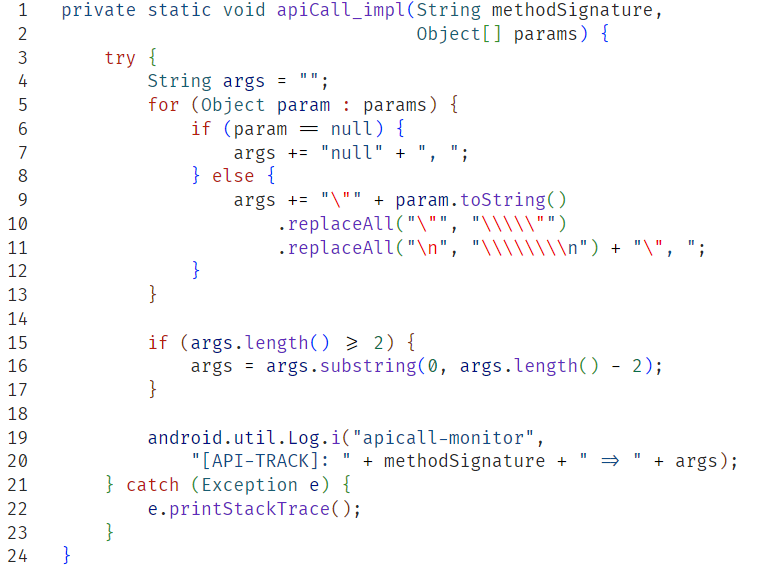
\includegraphics{img/api_monitor_impl.png}
    \caption{Source code of the implementation of the \textit{apiCall} method.}
    \label{lst:apitracker-monitor-impl}
\end{figure}

% \begin{lstlisting}[language=java, basicstyle={\small\ttfamily}, moredelim={[is][\color{red}]{STARTRC}{ENDRC}}, caption={Source code of the implementation of the \textit{apiCall} method.}\label{lst:apitracker-monitor-impl}]
% private static void apiCall_impl(String methodSignature, 
%                                  Object[] params) {
%     try {
%         String args = "";
%         for (Object param : params) {
%             if (param == null) {
%                 args += "null" + ", ";
%             } else {
%                 args += "\"" + param.toString()
%                     .replaceAll("\"", "\\\\\"")
%                     .replaceAll("\n", "\\\\\\\\n") + "\", ";
%             }
%         }

%         if (args.length() >= 2) {
%             args = args.substring(0, args.length() - 2);
%         }

%         android.util.Log.i("apicall-monitor", 
%             "[API-TRACK]: " + methodSignature + " => " + args);
%     } catch (Exception e) {
%         e.printStackTrace();
%     }
% }
% \end{lstlisting}

The \ic{methodSignature} string expects the signature of the method that was called. 

The \ic{params} array expects an array of Java objects, where each item represent an argument that was passed to the method at \ic{methodSignature}.

\subsection{sceneInstr class}

The \ic{sceneInstr} class is the main executable class. It's responsible for traversing the classes and methods of the provided APK using Soot to detect the sensitive API calls, and insert the \ic{Monitor.apiCall} call before the actual method invocation. It's also where the CLI arguments are parsed and inserted into the \ic{Options} class. It is built upon the base structure of other DroidFax's \ic{sceneInstr} classes.

In the following sections, the relevant methods of this class will be disclosed.

\subsubsection{The \ic{run()} method}

This method is responsible for being the entry point of the instrumentation process. It calls the \ic{init()} and \ic{instrument()} methods described below.

\subsubsection{The \ic{init()} method}

This method is responsible for loading the method signatures from the \ic{catsink} file, and associating them with their corresponding Android method category. The methods are then stored into an in-memory list, to be used by the instrumentation process.

It's also in this method that the \ic{Monitor} class is imported into the application package, and a reference for the \ic{apiCall} method is created.

\subsubsection{The \ic{instrument()} method}

This method is responsible for the actual instrumentation process. The first step is collecting all the classes in the application, and filtering them according to a defined pattern. We only want to capture method calls that are present in the original application code, and ignore the methods introduced by our own instrumentation (such as the \ic{apiCall} method).

After the classes are collected, we iterate over them checking their methods. If the body of the method contains an invocation of any method that's in our \ic{catsink} list, an invocation for the \ic{apiCall} tracker method is added using Soot. 

This procedure is made by:

\begin{enumerate}
    \item Collecting the number of arguments passed to the relevant method:
    
    This is done by using Soot's \ic{getArgCount()} method.
    \item Creating an empty array of Java objects: 
    
    Soot's \ic{generateLocal} method creates a local variable into the inspected method's body. This variable is typed as an array of \ic{Object}, and is initialized using a \ic{newArrayExpr}, that creates an empty array with a fixed length. The length of the array is equal to the number of arguments passed to the method that's being tracked. 

    All those steps are performed by creating Soots' statements that will be later inserted into the actual method body. An example of statement creation using Soot can be seen at Figure \ref{lst:apitracker-array-create}.
   
    \item Iterating through the arguments passed to the relevant method: 

    After the array is created, it's necessary to assign the values for their corresponding array positions. Every argument is a Soot \ic{Value} that can be referenced in an array position.

    However, not every argument will be assignable to an \ic{Object}. If a variable of a primitive type is passed to a Java \ic{Object} type, a JVM error will be raised and the application will stop running. For this reason, it was necessary to convert primitive types to their corresponding boxed types.

    \begin{enumerate}
        \item Handling primitive types

        Every Soot \ic{Value} instance have a \textit{type} property. This type is a subclass of a generic \ic{Type} class, such as \ic{PrimType}, \ic{RefLikeType}, etc.. For every argument, we check if their type is an instance of \ic{PrimType}, and if they are, we can find a \ic{RefLikeType} that represents the boxed type using the \ic{PrimType.boxedType()} method.

        After discovering the corresponding boxed type, it's necessary to perform the conversion. Firstly, a new local variable typed as the boxed type is generated, and then a verification is made to ensure that this type implements a \ic{valueOf} method receiving the primitive type as an argument. By default, every Java boxed type should implement this method, but the check is made to ensure that the instrumentation won't fail.

        After we're sure that the class implements the \ic{valueOf} method, a new invoke expression statement is created, along with the assignment statement for the created variable. The boxed value is now ready to be inserted into our array of objects, and this is also done by creating a new Soot statement.
    \end{enumerate}

    \item Create the invocation of the \ic{apiCall} method

    It's also necessary to create a statement to invoke our \ic{apiCall} method, that will log the tracked method and its collected arguments. This is done by creating a new \ic{invokeStmt} using the \ic{Monitor.apiCall} method reference (created before the instrumentation began) and passing the relevant method signature as a string, along with the newly created local variable representing the array of objects.

    \item Add the new statements to the method body

    After all the new statements are created, the last step is to add them to the method body. It's done by using Soot's \ic{insertBeforeNoRedirect} method, where a list of statements is passed to be inserted before an existing statement (in this case, before the relevant method invocation). A code example can be seen on listing \ref{lst:apitracker-stmt-insert}.
\end{enumerate}

\begin{figure}
    \centering
    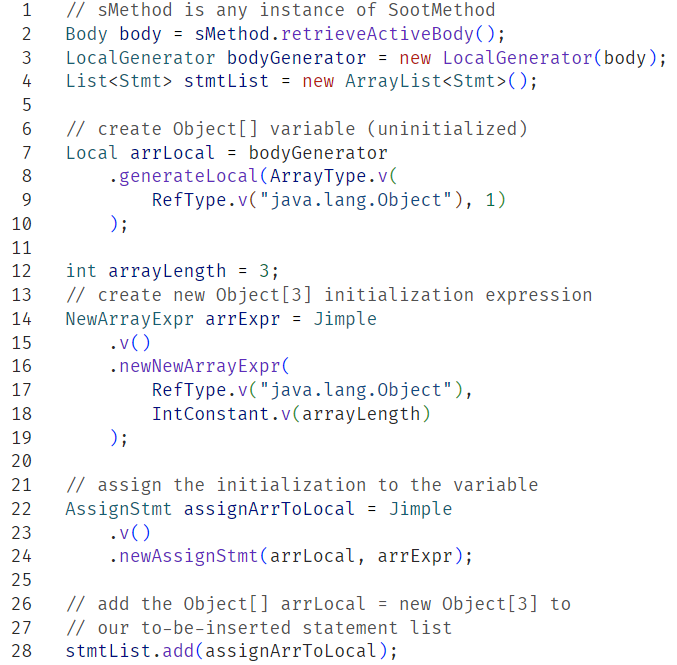
\includegraphics{img/apicall_array_create.png}
    \caption{Local variable creation, along with initialization statement and assignment statement using Soot}
    \label{lst:apitracker-array-create}
\end{figure}

% \begin{lstlisting}[language=java, basicstyle={\small\ttfamily}, moredelim={[is][\color{red}]{STARTRC}{ENDRC}}, caption={Local variable creation, along with initialization statement and assignment statement using Soot}\label{lst:apitracker-array-create}]
% // sMethod is any instance of SootMethod
% Body body = sMethod.retrieveActiveBody();
% LocalGenerator bodyGenerator = new LocalGenerator(body);
% List<Stmt> stmtList = new ArrayList<Stmt>();

% // create Object[] variable (uninitialized)
% Local arrLocal = bodyGenerator
%     .generateLocal(ArrayType.v(
%         RefType.v("java.lang.Object"), 1)
%     );

% int arrayLength = 3;
% // create new Object[3] initialization expression
% NewArrayExpr arrExpr = Jimple
%     .v()
%     .newNewArrayExpr(
%         RefType.v("java.lang.Object"), 
%         IntConstant.v(arrayLength)
%     );

% // assign the initialization to the variable
% AssignStmt assignArrToLocal = Jimple
%     .v()
%     .newAssignStmt(arrLocal, arrExpr);

% // add the Object[] arrLocal = new Object[3] to
% // our to-be-inserted statement list
% stmtList.add(assignArrToLocal);
% \end{lstlisting}

\begin{figure}
    \centering
    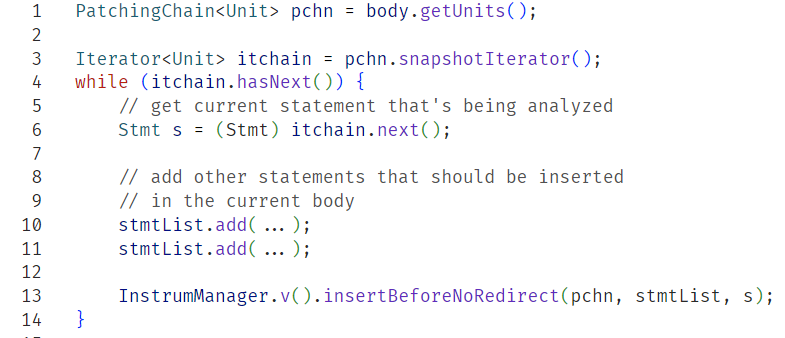
\includegraphics{img/apicall_insert.png}
    \caption{Statements insertion before an existing statement using Soot}
    \label{lst:apitracker-stmt-insert}
\end{figure}

% \begin{lstlisting}[language=java, basicstyle={\small\ttfamily}, moredelim={[is][\color{red}]{STARTRC}{ENDRC}}, caption={Statements insertion before an existing statement using Soot}\label{lst:apitracker-stmt-insert}]
% PatchingChain<Unit> pchn = body.getUnits();
				
% Iterator<Unit> itchain = pchn.snapshotIterator();    
% while (itchain.hasNext()) {
%     // get current statement that's being analyzed
%     Stmt s = (Stmt) itchain.next();

%     // add other statements that should be inserted
%     // in the current body
%     stmtList.add(...);
%     stmtList.add(...);
    
%     InstrumManager.v().insertBeforeNoRedirect(pchn, stmtList, s);
% }
% \end{lstlisting}

% describe how the things are created to capture the argumetns
% how the Monitor method is called
% how the primitive/null types are handled
% how its inserted before the method call

% cite how it was necessary to adapt the dynCG instr to have the apiTracker instr as an option

After this process is done and every method from every class is analyzed (and instrumented, if suitable), the instrumentation process is completed.

\section{DroidXP changes}

After the changes in the DroidFax code, it was necessary to perform a few adjustments on DroidXP\footnote{\url{https://github.com/droidxp/benchmark}} code. Those changes were focused on enabling the newly created instrumentation, and parsing its results to a Comma Separated Values (CSV) format.

Firstly, it was necessary to add an optional parameter in the DroidXP's CLI that enables our argument catching instrumentation. It was chosen to be \ic{-p}.

Then, if this flag was activated, it would pass the \ic{-monitorApiCalls} argument for the instrumentation at the first phase of the execution (instrumentation). 

At the second phase of the execution, a reboot simulation after the APK is installed on the emulator was also added. This was done to try to detect malware that had a flexible activation mechanism based on the device reboot. This reboot is done by issuing a specific Android intent, using the command at \ref{lst:droidxp-intent-reboot}. Also at the second phase, Android ADB's logcat\cite{noauthor_logcat_2023} starts listening for any logs tagged with ``apicall-monitor'', and saves them to a specific file for further parsing and analysis.

\begin{figure}
    \centering
    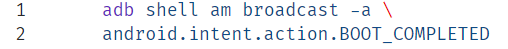
\includegraphics{img/adb-boot.png}
    \caption{Android Debug Bridge command command used to broadcast an Android intent through the system's activiy manager.}
    \label{lst:droidxp-intent-reboot}
\end{figure}

% \begin{lstlisting}[language=bash,caption={Android Debug Bridge command command used to broadcast an Android intent through the system's activiy manager.}\label{lst:droidxp-intent-reboot}]
%     adb shell am broadcast -a \
%     android.intent.action.BOOT_COMPLETED
% \end{lstlisting}

At the third phase of the execution, the logs captured in the logcat file for each executed APK are correctly parsed and converted to the CSV format.

It's also important to notice that some changes were made on the method that checks if the emulator has finished booting: in the previous version, sometimes the device wasn't ready yet when the countdown started. It was problematic on some executions, and a new command was added to check for a specific system property. The exact command is present on Figure \ref{lst:droidxp-wait-boot-complete}.

\begin{figure}
    \centering
    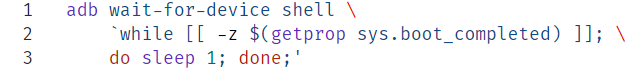
\includegraphics{img/adb-wait-device.png}
    \caption{Android Debug Bridge command command used to wait for the device boot to complete.}
    \label{lst:droidxp-wait-boot-complete}
\end{figure}
% \begin{lstlisting}[language=bash,caption={Android Debug Bridge command command used to wait for the device boot to complete.}\label{lst:droidxp-wait-boot-complete}]
%     adb wait-for-device shell \
%     `while [[ -z $(getprop sys.boot_completed) ]]; \
% do sleep 1; done;'
% \end{lstlisting}

With all the changes, it was possible to run the tool with a custom parameter, perform the newly implemented instrumentation process and collect the arguments passed for the sensitive methods of each analyzed app. The results were stored in the same way they were stored before, along with a new file called ``sensitiveMtdArgs.csv'', containing the methods and arguments that were captured during the execution of the application.

\section{Report generator}

After DroidXP's execution is finished, we're left with a lot of CSV files containing the sensitive methods called by both the malicious and benign versions of each app, along with the arguments passed to these methods. In order to compare the execution results, a Python script was created to parse the CSV files for each app version and compare the arguments. We call this script ``run assessment''\footnote{\url{https://github.com/droidxp/run-assessment-param}}.

The assessment is made by firstly grouping all the executions of the same version of the app in a HashSet, a data structure that only allows unique items. This is made to ensure that eventual execution differences will be minimized, and repetitions won't be counted. For each pair of apps, this result in two HashSets, one containing the sensitive methods and the arguments passed for them in the malicious APK execution, and another one with the same structure but for the benign APK execution. Methods that are called more than once, but with different arguments are two separate entries in the HashSet.

Then, the difference between those two sets is calculated, and we are left with a set of every method call that's executed in the malicious version, but is not executed in the benign version. The resulting method calls are filtered to only consider methods that are in a list of ``sensitive methods'', and the final result is saved into a CSV file. 